% !TEX TS-program = pdflatex
\documentclass[11pt]{article}

% -------------------- Packages --------------------
\usepackage[a4paper,margin=1in]{geometry}
\usepackage{amsmath,amssymb}
\usepackage[T1]{fontenc}
\usepackage{lmodern}
\usepackage{xcolor}
\usepackage{tcolorbox}
\tcbuselibrary{skins,breakable}
\usepackage{enumitem}
\usepackage{hyperref}
\usepackage{tikz}
\usetikzlibrary{calc,patterns,angles,quotes,intersections}

\pagestyle{empty}

% -------------------- Dark Theme Colors --------------------
\definecolor{bg}{HTML}{000000}
\definecolor{pairbg}{HTML}{121212}
\definecolor{solbg}{HTML}{0A0A0A}
\definecolor{border}{HTML}{2A2A2A}
\definecolor{text}{HTML}{FFFFFF}
\definecolor{muted}{HTML}{C9CDD3}
\definecolor{gold}{HTML}{FFD700}
\definecolor{green}{HTML}{4ADE80}
\definecolor{cyan}{HTML}{38BDF8}

\pagecolor{bg}
\color{text}

\hypersetup{
  colorlinks=true,
  linkcolor=cyan,
  urlcolor=cyan
}

\setlength{\parindent}{0pt}
\setlength{\parskip}{10pt}

\setlist[itemize]{left=1.4em,itemsep=6pt,topsep=6pt}
\setlist[enumerate]{left=1.6em,itemsep=4pt,topsep=4pt}

% Helps avoid small overfull lines
\setlength{\emergencystretch}{2em}

% -------------------- tcolorbox Base --------------------
\tcbset{
  enhanced,
  breakable,
  arc=12pt,
  boxrule=0.8pt,
  left=16pt,right=16pt,top=12pt,bottom=12pt
}

\newtcolorbox{QAPair}[1]{%
  colback=pairbg,
  colbacklower=solbg,
  colframe=border,
  coltext=text,
  title=\textcolor{gold}{\bfseries #1},
  fonttitle=\bfseries,
  coltitle=text,
  segmentation style={draw=border, dashed, line width=0.6pt},
}

\newtcolorbox{QuickBox}{%
  colback=pairbg,
  colframe=cyan,
  coltext=text,
  fontupper=\color{text},
  borderline north={4pt}{0pt}{cyan},
  arc=14pt,
  boxrule=0.8pt
}

% Helper for step headings
\newcommand{\Step}[1]{\textcolor{muted}{\textbf{Step #1:}}}

% -------------------- TikZ Styles --------------------
\tikzset{
  every picture/.style={line cap=round, line join=round},
  geom/.style={draw=muted, line width=0.95pt},
  strong/.style={draw=cyan, line width=1.05pt},
  helper/.style={draw=muted, dashed, line width=0.75pt},
  pt/.style={circle, fill=cyan, inner sep=1.2pt},
  lab/.style={text=text, font=\small},
  ang/.style={draw=cyan, line width=0.9pt},
  note/.style={text=muted, font=\small}
}

% Step + Diagram Macro
% Usage: \StepFig{1}{<text>}{<tikzpicture contents ONLY>}
\newcommand{\StepFig}[3]{%
  \Step{#1} #2\par\medskip
  \begin{center}
    \begin{tikzpicture}[scale=0.86]
      #3
    \end{tikzpicture}
  \end{center}
  \vspace{-2pt}
}

% tiny right-angle mark macro
\newcommand{\RightAngleMark}[2]{%
  % #1 = corner point (coordinate name), #2 = size
  \draw[ang] ($(#1)+(#2,0)$) -- ($(#1)+(#2,#2)$) -- ($(#1)+(0,#2)$);
}

% ============================================================
\begin{document}

\begin{center}
{\LARGE\bfseries \textcolor{gold}{Exercise 8.2 --- Solutions}}\\[-2pt]
\end{center}

\begin{QuickBox}
{\color{cyan}\bfseries Quick formulas (Right-triangle Trigonometry)}\par\medskip
% --- Added diagram for quick formulas (FIXED: no clashing) ---
{\color{muted}\small
\textbf{Diagram (labels used throughout):} Right angle at $C$. Hypotenuse $c=AB$, legs $a=BC$ and $b=AC$.
}\par\medskip

\begin{center}
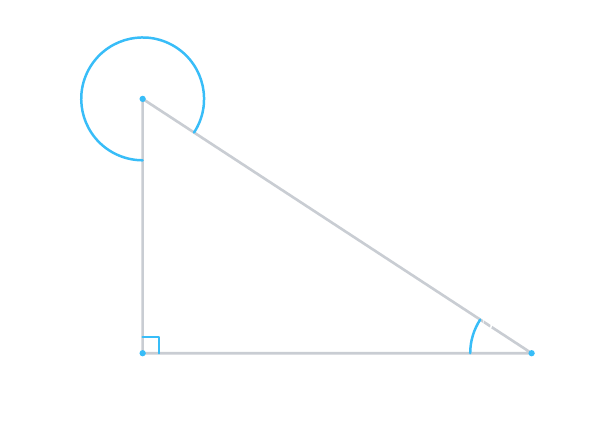
\begin{tikzpicture}[scale=0.95]
  \coordinate (C) at (0,0);
  \coordinate (B) at (5.2,0);
  \coordinate (A) at (0,3.4);

  \draw[geom] (A)--(C)--(B)--cycle;
  \RightAngleMark{C}{0.22}

  % points
  \fill[pt] (A) circle(1.2pt);
  \fill[pt] (B) circle(1.2pt);
  \fill[pt] (C) circle(1.2pt);

  % point labels (offset so they don't clash with angle arcs)
  \node[lab] at ($(A)+(-0.38,0.20)$) {$A$};
  \node[lab] at ($(B)+(0.35,-0.20)$) {$B$};
  \node[lab] at ($(C)+(-0.35,-0.20)$) {$C$};

  % side labels (pushed away from the sides)
  \node[lab] at ($(C)!0.5!(B)+(0,-0.50)$) {$a=BC$};
  \node[lab] at ($(A)!0.5!(C)+(-0.85,0)$) {$b=AC$};
  \node[lab] at ($(A)!0.5!(B)+(0.65,0.38)$) {$c=AB$};

  % angle arcs WITHOUT inline labels (we place labels manually)
  \pic[ang, angle radius=0.78cm, angle eccentricity=1.35] {angle = B--A--C};
  \node[lab] at ($(A)+(-0.05,0.70)$) {$\alpha$};

  \pic[ang, angle radius=0.78cm, angle eccentricity=1.35] {angle = A--B--C};
  \node[lab] at ($(B)+(-0.60,0.38)$) {$\beta$};

  % right angle label
  \node[lab] at ($(C)+(0.95,0.25)$) {$\gamma=90^\circ$};
\end{tikzpicture}
\end{center}

{\color{muted}\small Opposite $\alpha$ is $a$, and adjacent to $\alpha$ is $b$.}\par


\begin{itemize}
\item In $\triangle ABC$ with $\gamma=\angle C=90^\circ$ (right angle at $C$): $c=AB$ is \textbf{hypotenuse}, $a=BC$ and $b=AC$ are \textbf{legs}.
\item \textbf{SOH-CAH-TOA:}\quad $\sin\alpha=\dfrac{a}{c}$,\; $\cos\alpha=\dfrac{b}{c}$,\; $\tan\alpha=\dfrac{a}{b}$.
\item For $\beta$: \quad $\sin\beta=\dfrac{b}{c}$,\; $\cos\beta=\dfrac{a}{c}$,\; $\tan\beta=\dfrac{b}{a}$.
\item \textbf{Pythagoras:}\quad $a^2+b^2=c^2$.
\item \textbf{Complementary angles:}\quad $\alpha+\beta=90^\circ$.
\end{itemize}
\end{QuickBox}

% ============================================================
% Q1(i)
\begin{QAPair}{Question 1 (i)}
\textcolor{gold}{\bfseries Question:} In the right-angled triangle, $AB=15\,\text{m}$ and $\angle A=40^\circ$. Find $a$ and $b$.\par
\tcblower
\textcolor{green}{\bfseries Answer:}\par

\StepFig{1}{Draw and label the right triangle (right angle at $C$).}{%
  \coordinate (A) at (0,0);
  \coordinate (C) at (5,0);
  \coordinate (B) at (5,3.3);

  \draw[geom] (A)--(C)--(B)--cycle;
  \RightAngleMark{C}{0.22}

  \fill[pt] (A) circle(1.2pt) node[lab, below left] {$A$};
  \fill[pt] (B) circle(1.2pt) node[lab, above right] {$B$};
  \fill[pt] (C) circle(1.2pt) node[lab, below right] {$C$};

  \node[lab] at ($(A)!0.5!(B) + (-0.2,0.2)$) {$15\,\text{m}$};
  \node[lab] at ($(C)!0.5!(B) + (0.45,0)$) {$a$};
  \node[lab] at ($(A)!0.5!(C) + (0,-0.35)$) {$b$};

  \pic[ang, angle radius=0.7cm, "$40^\circ$"] {angle = C--A--B};
}

\[
\begin{aligned}
\Step{2}\;& \sin 40^\circ=\frac{a}{15}\Rightarrow a=15\sin40^\circ \approx 9.64\ \text{m}.\\
\Step{3}\;& \cos 40^\circ=\frac{b}{15}\Rightarrow b=15\cos40^\circ \approx 11.49\ \text{m}.\\
\Step{4}\;& \angle B=90^\circ-40^\circ=50^\circ.
\end{aligned}
\]
\textcolor{green}{\bfseries Final:}\quad $a\approx 9.64\,\text{m},\; b\approx 11.49\,\text{m}$ (and $\angle B=50^\circ$).
\end{QAPair}

% Q1(ii)
\begin{QAPair}{Question 1 (ii)}
\textcolor{gold}{\bfseries Question:} In the right-angled triangle, $AC=50\,\text{m}$ and $\angle B=35.5^\circ$. Find $a$ and $c$.\par
\tcblower
\textcolor{green}{\bfseries Answer:}\par

\StepFig{1}{Draw and label the triangle (right angle at $C$).}{%
  \coordinate (C) at (0,0);
  \coordinate (B) at (5,0);
  \coordinate (A) at (0,3.3);

  \draw[geom] (A)--(C)--(B)--cycle;
  \RightAngleMark{C}{0.22}

  \fill[pt] (A) circle(1.2pt) node[lab, above left] {$A$};
  \fill[pt] (B) circle(1.2pt) node[lab, below right] {$B$};
  \fill[pt] (C) circle(1.2pt) node[lab, below left] {$C$};

  \node[lab] at ($(A)!0.5!(C) + (-0.35,0)$) {$50\,\text{m}$};
  \node[lab] at ($(C)!0.5!(B) + (0,-0.35)$) {$a$};
  \node[lab] at ($(A)!0.5!(B) + (0.2,0.2)$) {$c$};

  \pic[ang, angle radius=0.8cm, "$35.5^\circ$"] {angle = A--B--C};
}

\[
\begin{aligned}
\Step{2}\;& \tan 35.5^\circ=\frac{50}{a}\Rightarrow a=\frac{50}{\tan35.5^\circ}\approx 70.10\ \text{m}.\\
\Step{3}\;& \sin 35.5^\circ=\frac{50}{c}\Rightarrow c=\frac{50}{\sin35.5^\circ}\approx 86.10\ \text{m}.\\
\Step{4}\;& \angle A=90^\circ-35.5^\circ=54.5^\circ.
\end{aligned}
\]
\textcolor{green}{\bfseries Final:}\quad $a\approx 70.10\,\text{m},\; c\approx 86.10\,\text{m}$ (and $\angle A=54.5^\circ$).
\end{QAPair}

% Q1(iii)
\begin{QAPair}{Question 1 (iii)}
\textcolor{gold}{\bfseries Question:} In the right-angled triangle, $AC=15\,\text{cm}$ and $CB=12.5\,\text{cm}$. Find $c$ and the acute angles.\par
\tcblower
\textcolor{green}{\bfseries Answer:}\par

\StepFig{1}{Draw and label the triangle (right angle at $C$).}{%
  \coordinate (C) at (0,0);
  \coordinate (B) at (5,0);
  \coordinate (A) at (0,3.2);

  \draw[geom] (A)--(C)--(B)--cycle;
  \RightAngleMark{C}{0.22}

  \fill[pt] (A) circle(1.2pt) node[lab, above left] {$A$};
  \fill[pt] (B) circle(1.2pt) node[lab, below right] {$B$};
  \fill[pt] (C) circle(1.2pt) node[lab, below left] {$C$};

  \node[lab] at ($(A)!0.5!(C) + (-0.40,0)$) {$15\,\text{cm}$};
  \node[lab] at ($(C)!0.5!(B) + (0,-0.35)$) {$12.5\,\text{cm}$};
  \node[lab] at ($(A)!0.5!(B) + (0.2,0.2)$) {$c$};
}

\[
\begin{aligned}
\Step{2}\;& c=\sqrt{15^2+12.5^2}=\sqrt{381.25}\approx 19.53\ \text{cm}.\\
\Step{3}\;& \tan \angle A=\frac{12.5}{15}\Rightarrow \angle A\approx 39.81^\circ.\\
\Step{4}\;& \angle B=90^\circ-\angle A\approx 50.19^\circ.
\end{aligned}
\]
\textcolor{green}{\bfseries Final:}\quad $c\approx 19.53\,\text{cm},\; \angle A\approx 39.81^\circ,\; \angle B\approx 50.19^\circ$.
\end{QAPair}

% ============================================================
% Q2(i)
\begin{QAPair}{Question 2 (i)}
\textcolor{gold}{\bfseries Question:} Solve $\triangle ABC$ where $\gamma=90^\circ$, $a=12\,\text{cm}$, $\beta=35^\circ$.\par
\tcblower
\textcolor{green}{\bfseries Answer:}\par

\StepFig{1}{Right triangle with $\gamma=90^\circ$ and $\beta=35^\circ$.}{%
  \coordinate (C) at (0,0);
  \coordinate (B) at (5,0);
  \coordinate (A) at (0,3.2);

  \draw[geom] (A)--(C)--(B)--cycle;
  \RightAngleMark{C}{0.22}

  \node[lab] at ($(C)!0.5!(B) + (0,-0.35)$) {$a=12$};
  \node[lab] at ($(A)!0.5!(C) + (-0.35,0)$) {$b$};
  \node[lab] at ($(A)!0.5!(B) + (0.2,0.2)$) {$c$};

  \pic[ang, angle radius=0.75cm, "$35^\circ$"] {angle = A--B--C};

  \fill[pt] (A) circle(1.2pt) node[lab, above left] {$A$};
  \fill[pt] (B) circle(1.2pt) node[lab, below right] {$B$};
  \fill[pt] (C) circle(1.2pt) node[lab, below left] {$C$};
}

\[
\begin{aligned}
\Step{2}\;& \alpha=90^\circ-\beta=55^\circ.\\
\Step{3}\;& c=\frac{12}{\cos35^\circ}\approx 14.65\ \text{cm}.\\
\Step{4}\;& b=12\tan35^\circ\approx 8.40\ \text{cm}.
\end{aligned}
\]
\textcolor{green}{\bfseries Final:}\quad $\alpha=55^\circ,\; b\approx 8.40\,\text{cm},\; c\approx 14.65\,\text{cm}$.
\end{QAPair}

% Q2(ii)
\begin{QAPair}{Question 2 (ii)}
\textcolor{gold}{\bfseries Question:} Solve $\triangle ABC$ where $\gamma=90^\circ$, $b=30\,\text{cm}$, $\alpha=25^\circ 35'$.\par
\tcblower
\textcolor{green}{\bfseries Answer:}\par

\StepFig{1}{Right triangle with given $\alpha$ and adjacent side $b=AC$.}{%
  \coordinate (C) at (0,0);
  \coordinate (B) at (5,0);
  \coordinate (A) at (0,3.2);

  \draw[geom] (A)--(C)--(B)--cycle;
  \RightAngleMark{C}{0.22}

  \node[lab] at ($(A)!0.5!(C) + (-0.35,0)$) {$b=30$};
  \node[lab] at ($(C)!0.5!(B) + (0,-0.35)$) {$a$};
  \node[lab] at ($(A)!0.5!(B) + (0.2,0.2)$) {$c$};

  \pic[ang, angle radius=0.8cm, "$25^\circ35'$"] {angle = B--A--C};

  \fill[pt] (A) circle(1.2pt) node[lab, above left] {$A$};
  \fill[pt] (B) circle(1.2pt) node[lab, below right] {$B$};
  \fill[pt] (C) circle(1.2pt) node[lab, below left] {$C$};
}

\[
\begin{aligned}
\Step{2}\;& \beta=90^\circ-\alpha=64^\circ25'.\\
\Step{3}\;& c=\frac{30}{\cos(25^\circ35')}\approx 33.26\ \text{cm}.\\
\Step{4}\;& a=30\tan(25^\circ35')\approx 14.36\ \text{cm}.
\end{aligned}
\]
\textcolor{green}{\bfseries Final:}\quad $\beta=64^\circ25',\; a\approx 14.36\,\text{cm},\; c\approx 33.26\,\text{cm}$.
\end{QAPair}

% Q2(iii)
\begin{QAPair}{Question 2 (iii)}
\textcolor{gold}{\bfseries Question:} Solve $\triangle ABC$ where $\gamma=90^\circ$, $a=50\,\text{cm}$, $b=25\,\text{cm}$.\par
\tcblower
\textcolor{green}{\bfseries Answer:}\par

\StepFig{1}{Right triangle with both legs given ($a$ and $b$).}{%
  \coordinate (C) at (0,0);
  \coordinate (B) at (5,0);
  \coordinate (A) at (0,3.2);

  \draw[geom] (A)--(C)--(B)--cycle;
  \RightAngleMark{C}{0.22}

  \node[lab] at ($(C)!0.5!(B) + (0,-0.35)$) {$a=50$};
  \node[lab] at ($(A)!0.5!(C) + (-0.35,0)$) {$b=25$};
  \node[lab] at ($(A)!0.5!(B) + (0.2,0.2)$) {$c$};

  \fill[pt] (A) circle(1.2pt) node[lab, above left] {$A$};
  \fill[pt] (B) circle(1.2pt) node[lab, below right] {$B$};
  \fill[pt] (C) circle(1.2pt) node[lab, below left] {$C$};
}

\[
\begin{aligned}
\Step{2}\;& c=\sqrt{50^2+25^2}=\sqrt{3125}\approx 55.90\ \text{cm}.\\
\Step{3}\;& \alpha=\tan^{-1}\!\left(\frac{50}{25}\right)\approx 63.43^\circ.\\
\Step{4}\;& \beta=90^\circ-\alpha\approx 26.57^\circ.
\end{aligned}
\]
\textcolor{green}{\bfseries Final:}\quad $c\approx 55.90\,\text{cm},\; \alpha\approx 63.43^\circ,\; \beta\approx 26.57^\circ$.
\end{QAPair}

% Q2(iv)
\begin{QAPair}{Question 2 (iv)}
\textcolor{gold}{\bfseries Question:} Solve $\triangle ABC$ where $\gamma=90^\circ$, $a=30\,\text{cm}$, $c=40\,\text{cm}$.\par
\tcblower
\textcolor{green}{\bfseries Answer:}\par

\StepFig{1}{Right triangle with hypotenuse $c$ and one leg $a$.}{%
  \coordinate (C) at (0,0);
  \coordinate (B) at (5,0);
  \coordinate (A) at (0,3.2);

  \draw[geom] (A)--(C)--(B)--cycle;
  \RightAngleMark{C}{0.22}

  \node[lab] at ($(C)!0.5!(B) + (0,-0.35)$) {$a=30$};
  \node[lab] at ($(A)!0.5!(C) + (-0.35,0)$) {$b$};
  \node[lab] at ($(A)!0.5!(B) + (0.2,0.2)$) {$c=40$};

  \fill[pt] (A) circle(1.2pt) node[lab, above left] {$A$};
  \fill[pt] (B) circle(1.2pt) node[lab, below right] {$B$};
  \fill[pt] (C) circle(1.2pt) node[lab, below left] {$C$};
}

\[
\begin{aligned}
\Step{2}\;& b=\sqrt{40^2-30^2}=\sqrt{700}\approx 26.46\ \text{cm}.\\
\Step{3}\;& \beta=\cos^{-1}\!\left(\frac{30}{40}\right)\approx 41.41^\circ.\\
\Step{4}\;& \alpha=90^\circ-\beta\approx 48.59^\circ.
\end{aligned}
\]
\textcolor{green}{\bfseries Final:}\quad $b\approx 26.46\,\text{cm},\; \beta\approx 41.41^\circ,\; \alpha\approx 48.59^\circ$.
\end{QAPair}

% Q2(v)
\begin{QAPair}{Question 2 (v)}
\textcolor{gold}{\bfseries Question:} Solve $\triangle ABC$ where $\gamma=90^\circ$, $a=24\,\text{cm}$, $\alpha=36^\circ 15'$.\par
\tcblower
\textcolor{green}{\bfseries Answer:}\par

\StepFig{1}{Right triangle with given $\alpha$ and opposite side $a$.}{%
  \coordinate (C) at (0,0);
  \coordinate (B) at (5,0);
  \coordinate (A) at (0,3.2);

  \draw[geom] (A)--(C)--(B)--cycle;
  \RightAngleMark{C}{0.22}

  \node[lab] at ($(C)!0.5!(B) + (0,-0.35)$) {$a=24$};
  \node[lab] at ($(A)!0.5!(C) + (-0.35,0)$) {$b$};
  \node[lab] at ($(A)!0.5!(B) + (0.2,0.2)$) {$c$};

  \pic[ang, angle radius=0.8cm, "$36^\circ15'$"] {angle = B--A--C};

  \fill[pt] (A) circle(1.2pt) node[lab, above left] {$A$};
  \fill[pt] (B) circle(1.2pt) node[lab, below right] {$B$};
  \fill[pt] (C) circle(1.2pt) node[lab, below left] {$C$};
}

\[
\begin{aligned}
\Step{2}\;& \beta=90^\circ-\alpha=53^\circ45'.\\
\Step{3}\;& c=\frac{24}{\sin(36^\circ15')}\approx 40.59\ \text{cm}.\\
\Step{4}\;& b=c\cos(36^\circ15')\approx 32.73\ \text{cm}.
\end{aligned}
\]
\textcolor{green}{\bfseries Final:}\quad $\beta=53^\circ45',\; b\approx 32.73\,\text{cm},\; c\approx 40.59\,\text{cm}$.
\end{QAPair}

% Q2(vi)
\begin{QAPair}{Question 2 (vi)}
\textcolor{gold}{\bfseries Question:} Solve $\triangle ABC$ where $\gamma=90^\circ$, $b=10\,\text{cm}$, $\alpha=70.5^\circ$.\par
\tcblower
\textcolor{green}{\bfseries Answer:}\par

\StepFig{1}{Right triangle with given $\alpha$ and adjacent side $b$.}{%
  \coordinate (C) at (0,0);
  \coordinate (B) at (5,0);
  \coordinate (A) at (0,3.2);

  \draw[geom] (A)--(C)--(B)--cycle;
  \RightAngleMark{C}{0.22}

  \node[lab] at ($(A)!0.5!(C) + (-0.35,0)$) {$b=10$};
  \node[lab] at ($(C)!0.5!(B) + (0,-0.35)$) {$a$};
  \node[lab] at ($(A)!0.5!(B) + (0.2,0.2)$) {$c$};

  \pic[ang, angle radius=0.8cm, "$70.5^\circ$"] {angle = B--A--C};

  \fill[pt] (A) circle(1.2pt) node[lab, above left] {$A$};
  \fill[pt] (B) circle(1.2pt) node[lab, below right] {$B$};
  \fill[pt] (C) circle(1.2pt) node[lab, below left] {$C$};
}

\[
\begin{aligned}
\Step{2}\;& \beta=90^\circ-\alpha=19.5^\circ.\\
\Step{3}\;& a=10\tan(70.5^\circ)\approx 28.26\ \text{cm}.\\
\Step{4}\;& c=\frac{10}{\cos(70.5^\circ)}\approx 29.98\ \text{cm}.
\end{aligned}
\]
\textcolor{green}{\bfseries Final:}\quad $\beta=19.5^\circ,\; a\approx 28.26\,\text{cm},\; c\approx 29.98\,\text{cm}$.
\end{QAPair}

% ============================================================
% Q3
\begin{QAPair}{Question 3}
\textcolor{gold}{\bfseries Question:} A tower casts a shadow $20\,\text{m}$ long when the angle of elevation of the sun is $65^\circ$. How tall is the tower?\par
\tcblower
\textcolor{green}{\bfseries Answer:}\par

\StepFig{1}{Model as a right triangle (height vs. shadow).}{%
  \coordinate (A) at (0,0);   % base
  \coordinate (T) at (0,3.2); % top
  \coordinate (S) at (5.0,0); % shadow end

  \draw[geom] (A)--(S);
  \draw[geom] (A)--(T);
  \draw[geom] (T)--(S);
  \RightAngleMark{A}{0.22}

  \node[lab] at ($(A)!0.5!(T)+(-0.45,0)$) {$h$};
  \node[lab] at ($(A)!0.5!(S)+(0,-0.35)$) {$20$ m};

  \pic[ang, angle radius=0.85cm, "$65^\circ$"] {angle = A--S--T};

  \fill[pt] (A) circle(1.2pt) node[lab, below] {Base};
  \fill[pt] (T) circle(1.2pt) node[lab, left] {Top};
  \fill[pt] (S) circle(1.2pt) node[lab, below] {Shadow end};
}

\[
\Step{2}\; \tan 65^\circ=\frac{h}{20}\Rightarrow h=20\tan65^\circ\approx 42.89\ \text{m}.
\]
\textcolor{green}{\bfseries Final:}\quad The tower is approximately $\boxed{42.89\ \text{m}}$ tall.
\end{QAPair}

% ============================================================
% Q4
\begin{QAPair}{Question 4}
\textcolor{gold}{\bfseries Question:} Arif is standing on top of a cliff $105\,\text{m}$ above a lake. The angle of depression to a boat is $42^\circ$. How far is the boat from Arif?\par
\tcblower
\textcolor{green}{\bfseries Answer:}\par
\StepFig{1}{Angle of depression equals angle of elevation ($42^\circ$).}{%
  \coordinate (T) at (0,3.6); % top (Arif)
  \coordinate (F) at (0,0);   % foot of cliff
  \coordinate (B) at (5.4,0); % boat
  \coordinate (R) at ($(T)+(6.0,0)$); % horizontal reference from T

  \draw[geom] (F)--(B);
  \draw[geom] (F)--(T);
  \draw[geom] (T)--(B);

  \RightAngleMark{F}{0.22}

  \node[lab] at ($(F)!0.5!(T)+(-0.55,0)$) {$105$ m};
  \node[lab] at ($(T)!0.5!(B)+(0.25,0.25)$) {$d$};

  % horizontal from top for depression
  \draw[helper] (T)--(R);

  % angle arc (no inline label)
  \pic[ang, angle radius=0.85cm, angle eccentricity=1.25] {angle = R--T--B};

  % manual label placed away from point label
  \node[lab] at ($(T)+(1.15,0.45)$) {$42^\circ$};

  \fill[pt] (T) circle(1.2pt) node[lab, left, xshift=-2pt] {Arif};
  \fill[pt] (B) circle(1.2pt) node[lab, below] {Boat};
  \fill[pt] (F) circle(1.2pt) node[lab, below left] {Foot};
}


\[
\Step{2}\; \sin 42^\circ=\frac{105}{d}\Rightarrow d=\frac{105}{\sin42^\circ}\approx 156.94\ \text{m}.
\]
\textcolor{green}{\bfseries Final:}\quad The boat is approximately $\boxed{156.94\ \text{m}}$ from Arif (line-of-sight).\par
{\color{muted}\small (Horizontal distance from the foot: $x=\frac{105}{\tan42^\circ}\approx 116.59\,\text{m}$.)}
\end{QAPair}

% ============================================================
% Q5
\begin{QAPair}{Question 5}
\textcolor{gold}{\bfseries Question:} A ladder $20$ ft long leans against a building. If the angle between the ladder and the ground is $75^\circ$, how far is the bottom of the ladder from the base of the building?\par
\tcblower
\textcolor{green}{\bfseries Answer:}\par

\StepFig{1}{Adjacent side is the ground distance.}{%
  \coordinate (G) at (0,0);   % wall base
  \coordinate (B) at (5.3,0); % ladder bottom
  \coordinate (T) at (0,3.6); % contact point on wall

  \draw[geom] (G)--(B);
  \draw[geom] (G)--(T);
  \draw[geom] (T)--(B);

  \RightAngleMark{G}{0.22}

  \node[lab] at ($(T)!0.5!(B)+(0.2,0.2)$) {$20$ ft};
  \node[lab] at ($(G)!0.5!(B)+(0,-0.35)$) {$x$};

  \pic[ang, angle radius=0.85cm, "$75^\circ$"] {angle = T--B--G};

  \fill[pt] (G) circle(1.2pt) node[lab, below left] {Wall};
  \fill[pt] (T) circle(1.2pt) node[lab, left] {Top};
  \fill[pt] (B) circle(1.2pt) node[lab, below] {Bottom};
}

\[
\Step{2}\; \cos 75^\circ=\frac{x}{20}\Rightarrow x=20\cos75^\circ\approx 5.18\ \text{ft}.
\]
\textcolor{green}{\bfseries Final:}\quad The bottom is about $\boxed{5.18\ \text{ft}}$ from the building.
\end{QAPair}

% ============================================================
% Q6
\begin{QAPair}{Question 6}
\textcolor{gold}{\bfseries Question:} Uzma is standing $50$ meters from a hot air balloon. The angle of elevation to the top is $28^\circ$. Find the height of the balloon.\par
\tcblower
\textcolor{green}{\bfseries Answer:}\par

\StepFig{1}{Height = opposite, ground distance = adjacent.}{%
  \coordinate (U) at (0,0);
  \coordinate (F) at (5.5,0);
  \coordinate (T) at (5.5,3.3);

  \draw[geom] (U)--(F);
  \draw[geom] (F)--(T);
  \draw[geom] (U)--(T);

  \RightAngleMark{F}{0.22}

  \node[lab] at ($(U)!0.5!(F)+(0,-0.35)$) {$50$ m};
  \node[lab] at ($(F)!0.5!(T)+(0.45,0)$) {$h$};

  \pic[ang, angle radius=0.85cm, "$28^\circ$"] {angle = F--U--T};

  \fill[pt] (U) circle(1.2pt) node[lab, below] {Uzma};
  \fill[pt] (F) circle(1.2pt) node[lab, below] {Foot};
  \fill[pt] (T) circle(1.2pt) node[lab, right] {Top};
}

\[
\Step{2}\; \tan 28^\circ=\frac{h}{50}\Rightarrow h=50\tan28^\circ\approx 26.60\ \text{m}.
\]
\textcolor{green}{\bfseries Final:}\quad The balloon is approximately $\boxed{26.60\ \text{m}}$ high.
\end{QAPair}

% ============================================================
% Q7
\begin{QAPair}{Question 7}
\textcolor{gold}{\bfseries Question:} A man is in a boat floating $175$ feet from the base of a $200$-foot cliff. What is the angle of depression between the cliff and the boat?\par
\tcblower
\textcolor{green}{\bfseries Answer:}\par

\StepFig{1}{Angle of depression from the top equals angle of elevation from the boat.}{%
  \coordinate (F) at (0,0);
  \coordinate (T) at (0,3.6);
  \coordinate (B) at (5.3,0);
  \coordinate (TH) at ($(T)+(5.9,0)$);

  \draw[geom] (F)--(B);
  \draw[geom] (F)--(T);
  \draw[geom] (T)--(B);
  \RightAngleMark{F}{0.22}

  \node[lab] at ($(F)!0.5!(T)+(-0.45,0)$) {$200$ ft};
  \node[lab] at ($(F)!0.5!(B)+(0,-0.35)$) {$175$ ft};

  \draw[helper] (T)--(TH);
  \pic[ang, angle radius=0.85cm, "$\theta$"] {angle = TH--T--B};

  \fill[pt] (T) circle(1.2pt) node[lab, left] {Top};
  \fill[pt] (F) circle(1.2pt) node[lab, below left] {Base};
  \fill[pt] (B) circle(1.2pt) node[lab, below] {Boat};
}

\[
\Step{2}\; \tan\theta=\frac{200}{175}\Rightarrow \theta=\tan^{-1}\!\left(\frac{200}{175}\right)\approx 48.81^\circ.
\]
\textcolor{green}{\bfseries Final:}\quad Angle of depression $\approx \boxed{48.81^\circ}$.
\end{QAPair}

% ============================================================
% Q8
\begin{QAPair}{Question 8}
\textcolor{gold}{\bfseries Question:} A flagpole casts a shadow $40$ feet long when the angle of elevation to the sun is $31^\circ$. How tall is the flagpole?\par
\tcblower
\textcolor{green}{\bfseries Answer:}\par

\StepFig{1}{Height of pole = opposite; shadow = adjacent.}{%
  \coordinate (A) at (0,0);   % base of pole
  \coordinate (T) at (0,3.2); % top of pole
  \coordinate (S) at (6.2,0); % end of shadow

  \draw[geom] (A)--(S);
  \draw[geom] (A)--(T);
  \draw[geom] (T)--(S);
  \RightAngleMark{A}{0.22}

  \node[lab] at ($(A)!0.5!(S)+(0,-0.35)$) {$40$ ft};
  \node[lab] at ($(A)!0.5!(T)+(-0.45,0)$) {$h$};

  \pic[ang, angle radius=0.9cm, "$31^\circ$"] {angle = A--S--T};

  \fill[pt] (A) circle(1.2pt) node[lab, below] {Pole base};
  \fill[pt] (T) circle(1.2pt) node[lab, left] {Top};
  \fill[pt] (S) circle(1.2pt) node[lab, below] {Shadow end};
}

\[
\Step{2}\; \tan31^\circ=\frac{h}{40}\Rightarrow h=40\tan31^\circ\approx 24.03\ \text{ft}.
\]
\textcolor{green}{\bfseries Final:}\quad Height $\approx \boxed{24.03\ \text{ft}}$.
\end{QAPair}

% ============================================================
% Q9
\begin{QAPair}{Question 9}
\textcolor{gold}{\bfseries Question:} A straight waterslide is $175$ feet above the ground and is $200$ feet long. What is the angle of depression to the bottom of the slide?\par
\tcblower
\textcolor{green}{\bfseries Answer:}\par

\StepFig{1}{The slide is the hypotenuse; height is opposite the depression angle.}{%
  \coordinate (T) at (0,3.6);
  \coordinate (B) at (6.2,0);
  \coordinate (F) at (0,0);
  \coordinate (TH) at ($(T)+(6.6,0)$);

  \draw[geom] (F)--(B);
  \draw[geom] (F)--(T);
  \draw[geom] (T)--(B);

  \RightAngleMark{F}{0.22}
  \node[lab] at ($(F)!0.5!(T)+(-0.45,0)$) {$175$ ft};
  \node[lab] at ($(T)!0.5!(B)+(0.2,0.2)$) {$200$ ft};

  \draw[helper] (T)--(TH);
  \pic[ang, angle radius=0.85cm, "$\theta$"] {angle = TH--T--B};

  \fill[pt] (T) circle(1.2pt) node[lab, left] {Top};
  \fill[pt] (B) circle(1.2pt) node[lab, below] {Bottom};
  \fill[pt] (F) circle(1.2pt) node[lab, below left] {};
}

\[
\Step{2}\; \sin\theta=\frac{175}{200}=0.875\Rightarrow \theta=\sin^{-1}(0.875)\approx 61.05^\circ.
\]
\textcolor{green}{\bfseries Final:}\quad Angle of depression $\approx \boxed{61.05^\circ}$.
\end{QAPair}

% ============================================================
% Q10
\begin{QAPair}{Question 10}
\textcolor{gold}{\bfseries Question:} Zain walks exactly $50\,\text{m}$ from the base of a tree and sees the angle of elevation to the top as $33^\circ$. How tall is the tree?\par
\tcblower
\textcolor{green}{\bfseries Answer:}\par

\StepFig{1}{Ground distance = adjacent; tree height = opposite.}{%
  \coordinate (Z) at (0,0);    % Zain
  \coordinate (B) at (6.0,0);  % tree base
  \coordinate (T) at (6.0,3.4);% tree top

  \draw[geom] (Z)--(B);
  \draw[geom] (B)--(T);
  \draw[geom] (Z)--(T);

  \RightAngleMark{B}{0.22}

  \node[lab] at ($(Z)!0.5!(B)+(0,-0.35)$) {$50$ m};
  \node[lab] at ($(B)!0.5!(T)+(0.45,0)$) {$h$};

  \pic[ang, angle radius=0.9cm, "$33^\circ$"] {angle = B--Z--T};

  \fill[pt] (Z) circle(1.2pt) node[lab, below] {Zain};
  \fill[pt] (B) circle(1.2pt) node[lab, below] {Tree base};
  \fill[pt] (T) circle(1.2pt) node[lab, right] {Top};
}

\[
\Step{2}\; \tan33^\circ=\frac{h}{50}\Rightarrow h=50\tan33^\circ\approx 32.47\ \text{m}.
\]
\textcolor{green}{\bfseries Final:}\quad The tree is about $\boxed{32.47\ \text{m}}$ tall.
\end{QAPair}

% ============================================================
% Q11
\begin{QAPair}{Question 11}
\textcolor{gold}{\bfseries Question:} From a $100\,\text{m}$ observation tower on the beach, the angle of depression of a whale is $7^\circ$. How far is the whale from the shoreline?\par
\tcblower
\textcolor{green}{\bfseries Answer:}\par

\StepFig{1}{Use angle of depression from the top (measured from the horizontal).}{%
  \coordinate (F) at (0,0);      % tower base
  \coordinate (T) at (0,3.6);    % tower top
  \coordinate (W) at (7.2,0);    % whale position
  \coordinate (TH) at ($(T)+(7.8,0)$); % horizontal reference

  \draw[geom] (F)--(W);
  \draw[geom] (F)--(T);
  \draw[geom] (T)--(W);
  \RightAngleMark{F}{0.22}

  \node[lab] at ($(F)!0.5!(T)+(-0.45,0)$) {$100$ m};
  \node[lab] at ($(F)!0.5!(W)+(0,-0.35)$) {$x$};

  \draw[helper] (T)--(TH);
  \pic[ang, angle radius=0.9cm, "$7^\circ$"] {angle = TH--T--W};

  \fill[pt] (T) circle(1.2pt) node[lab, left] {Tower top};
  \fill[pt] (F) circle(1.2pt) node[lab, below left] {Shoreline};
  \fill[pt] (W) circle(1.2pt) node[lab, below] {Whale};
}

\[
\Step{2}\; \tan7^\circ=\frac{100}{x}\Rightarrow x=\frac{100}{\tan7^\circ}\approx 814.49\ \text{m}.
\]
\textcolor{green}{\bfseries Final:}\quad The whale is approximately $\boxed{814.49\ \text{m}}$ from the shoreline.
\end{QAPair}

% ============================================================
% Q12
\begin{QAPair}{Question 12}
\textcolor{gold}{\bfseries Question:} Urooba sits midway between two trees $100\,\text{m}$ apart. The angles of elevation to the tops are $13^\circ$ and $18^\circ$. How much taller is one tree than the other?\par
\tcblower
\textcolor{green}{\bfseries Answer:}\par

\StepFig{1}{She is $50$ m from each tree (midpoint).}{%
  \coordinate (L) at (0,0);
  \coordinate (R) at (8.0,0);
  \coordinate (M) at (4.0,0);

  \coordinate (TL) at (0,2.3);
  \coordinate (TR) at (8.0,3.4);

  \draw[geom] (L)--(R);
  \draw[geom] (L)--(TL);
  \draw[geom] (R)--(TR);

  \draw[strong] (M)--(TL);
  \draw[strong] (M)--(TR);

  \RightAngleMark{L}{0.22}
  \RightAngleMark{R}{0.22}

  \node[lab] at ($(L)!0.5!(M)+(0,-0.35)$) {$50$ m};
  \node[lab] at ($(M)!0.5!(R)+(0,-0.35)$) {$50$ m};

  \node[lab] at ($(L)!0.5!(TL)+(-0.45,0)$) {$h_1$};
  \node[lab] at ($(R)!0.5!(TR)+(0.45,0)$) {$h_2$};

  \pic[ang, angle radius=0.9cm, "$13^\circ$"] {angle = L--M--TL};
  \pic[ang, angle radius=1.2cm, "$18^\circ$"] {angle = R--M--TR};

  \fill[pt] (M) circle(1.2pt) node[lab, below] {Urooba};
  \fill[pt] (L) circle(1.2pt) node[lab, below] {Tree 1};
  \fill[pt] (R) circle(1.2pt) node[lab, below] {Tree 2};
}

Since she is midway, she is $50$ m from each tree.
\[
\begin{aligned}
\Step{2}\;& h_1=50\tan13^\circ,\qquad h_2=50\tan18^\circ.\\
\Step{3}\;& \Delta h=h_2-h_1=50(\tan18^\circ-\tan13^\circ)\approx 4.70\ \text{m}.
\end{aligned}
\]
\textcolor{green}{\bfseries Final:}\quad One tree is about $\boxed{4.70\ \text{m}}$ taller than the other.
\end{QAPair}

% ============================================================
% Q13
\begin{QAPair}{Question 13}
\textcolor{gold}{\bfseries Question:} From the same point on the ground, the angle of elevation of the top of a tree $T$ is $27^\circ$. The angle of elevation of a hawk $H$ flying directly above the tree is $43^\circ$. The tree is $12.7\,\text{m}$ tall. How high is the hawk above the ground?\par
\tcblower
\textcolor{green}{\bfseries Answer:}\par

\StepFig{1}{Two sight lines from the same point: to tree top and to hawk above it.}{%
  \coordinate (P) at (0,0);
  \coordinate (D) at (6.0,0);
  \coordinate (T) at (6.0,2.7);
  \coordinate (H) at (6.0,4.3);
  \coordinate (X) at (7.0,0);

  \draw[geom] (P)--(X);
  \draw[geom] (P)--(D);
  \draw[geom] (D)--(H);
  \draw[strong] (P)--(T);
  \draw[strong] (P)--(H);

  \RightAngleMark{D}{0.22}

  \node[lab] at ($(D)!0.5!(T)+(-0.65,0)$) {$12.7$ m};
  \node[lab] at ($(P)!0.5!(D)+(0,-0.50)$) {$d$};
  \node[lab] at ($(T)+(0.35,0.05)$) {Tree top};
  \node[lab] at ($(H)+(0.35,0.05)$) {Hawk};

  \fill[pt] (P) circle(1.2pt) node[lab, below left, xshift=-2pt, yshift=-2pt] {Point};
  \fill[pt] (D) circle(1.2pt) node[lab, below] {Tree base};
  \fill[pt] (T) circle(1.2pt);
  \fill[pt] (H) circle(1.2pt);

  % bigger separation: inner vs outer radius further apart
  \pic[ang, angle radius=0.75cm, angle eccentricity=1.25] {angle = X--P--T}; % 27°
  \pic[ang, angle radius=1.45cm, angle eccentricity=1.12] {angle = X--P--H}; % 43°

  % manual labels moved further apart
  \node[lab] at ($(P)+(1.15,0.14)$) {$27^\circ$};
  \node[lab] at ($(P)+(1.25,0.78)$) {$43^\circ$};
}



\[
\begin{aligned}
\Step{2}\;& \tan27^\circ=\frac{12.7}{d}\Rightarrow d=\frac{12.7}{\tan27^\circ}.\\
\Step{3}\;& \tan43^\circ=\frac{h}{d}\Rightarrow h=\frac{12.7\tan43^\circ}{\tan27^\circ}\approx 23.24\ \text{m}.
\end{aligned}
\]
\textcolor{green}{\bfseries Final:}\quad The hawk is approximately $\boxed{23.24\ \text{m}}$ above the ground.\par
{\color{muted}\small (So it is about $23.24-12.7\approx 10.54$ m above the top of the tree.)}
\end{QAPair}

% ============================================================
% Q14
\begin{QAPair}{Question 14}
\textcolor{gold}{\bfseries Question:} A falcon $F$ is on a tree of height $15\,\text{m}$. The angles of depression to a chipmunk $C$ and squirrel $S$ are $47^\circ$ and $36^\circ$. How far apart are the animals on the ground?\par
\tcblower
\textcolor{green}{\bfseries Answer:}\par

\StepFig{1}{Smaller depression angle $\Rightarrow$ farther animal.}{%
  \coordinate (G) at (0,0);
  \coordinate (F) at (0,3.6);
  \coordinate (C) at (3.2,0);
  \coordinate (S) at (5.6,0);
  \coordinate (R) at ($(F)+(6.4,0)$); % horizontal reference to the right

  \draw[geom] (G)--(S);
  \draw[geom] (G)--(F);
  \RightAngleMark{G}{0.22}

  \draw[strong] (F)--(C);
  \draw[strong] (F)--(S);

  % horizontal reference for depression
  \draw[helper] (F)--(R);

  \node[lab] at ($(G)!0.5!(F)+(-0.60,0)$) {$15$ m};
  \node[note] at (3.2,-0.75) {$CS=GS-GC$};

  \fill[pt] (F) circle(1.2pt) node[lab, left] {$F$};
  \fill[pt] (G) circle(1.2pt) node[lab, below left] {$G$};
  \fill[pt] (C) circle(1.2pt) node[lab, below] {$C$};
  \fill[pt] (S) circle(1.2pt) node[lab, below] {$S$};

  % ---- CLOCKWISE depression arcs (manual) ----
  % 47° to chipmunk C (inner arc)
  \draw[ang] (F) ++(0.85,0) arc[start angle=0, end angle=-47, radius=0.85];
  \node[lab] at ($(F)+(0.95,-0.42)$) {$47^\circ$};

  % 36° to squirrel S (outer arc)
  \draw[ang] (F) ++(1.25,0) arc[start angle=0, end angle=-36, radius=1.25];
  \node[lab] at ($(F)+(1.35,-0.22)$) {$36^\circ$};
}




\[
\begin{aligned}
\Step{2}\;& GS=\frac{15}{\tan36^\circ},\qquad GC=\frac{15}{\tan47^\circ}.\\
\Step{3}\;& CS=\frac{15}{\tan36^\circ}-\frac{15}{\tan47^\circ}\approx 6.66\ \text{m}.
\end{aligned}
\]
\textcolor{green}{\bfseries Final:}\quad The animals are about $\boxed{6.66\ \text{m}}$ apart.
\end{QAPair}

% ============================================================
% Q15
\begin{QAPair}{Question 15}
\textcolor{gold}{\bfseries Question:} Two guy wires support a flagpole $FH$. The first wire is $11.2\,\text{m}$ long and has an angle of elevation $39^\circ$. The second wire has an angle of elevation $47^\circ$. How tall is the flagpole?\par
\tcblower
\textcolor{green}{\bfseries Answer:}\par

\StepFig{1}{Use the first wire to find $EH$, then use $47^\circ$ to get $FH$.}{%
  \coordinate (E) at (0,0);
  \coordinate (H) at (6.0,0);
  \coordinate (F) at (6.0,3.7);
  \coordinate (G) at (6.0,2.6);

  \draw[geom] (E)--(H);
  \draw[geom] (H)--(F);
  \draw[strong] (E)--(G);
  \draw[strong] (E)--(F);

  \RightAngleMark{H}{0.22}

  \node[lab] at ($(E)!0.5!(G)+(0.35,0.30)$) {$11.2$ m};
  \node[lab] at ($(H)!0.5!(F)+(0.55,0)$) {$FH$};

  \fill[pt] (E) circle(1.2pt) node[lab, below left, xshift=-3pt, yshift=-2pt] {$E$};
  \fill[pt] (H) circle(1.2pt) node[lab, below] {$H$};
  \fill[pt] (F) circle(1.2pt) node[lab, right] {$F$};
  \fill[pt] (G) circle(1.2pt) node[lab, right] {$G$};

  % bigger separation: inner vs outer radius further apart
  \pic[ang, angle radius=0.75cm, angle eccentricity=1.25] {angle = H--E--G}; % 39°
  \pic[ang, angle radius=1.40cm, angle eccentricity=1.12] {angle = H--E--F}; % 47°

  % manual labels moved further apart
  \node[lab] at ($(E)+(1.15,0.14)$) {$39^\circ$};
  \node[lab] at ($(E)+(1.22,0.76)$) {$47^\circ$};
}


\[
\begin{aligned}
\Step{2}\;& EH=11.2\cos39^\circ\approx 8.70\ \text{m}.\\
\Step{3}\;& FH=EH\tan47^\circ\approx 9.33\ \text{m}.
\end{aligned}
\]
\textcolor{green}{\bfseries Final:}\quad The flagpole is approximately $\boxed{9.33\ \text{m}}$ tall.
\end{QAPair}

\end{document}
